\input{configuration}

\title{Lecture 16 --- Query Processing }

\author{Jeff Zarnett \\ \small \texttt{jzarnett@uwaterloo.ca}}
\institute{Department of Electrical and Computer Engineering \\
  University of Waterloo}
\date{\today}


\begin{document}

\begin{frame}
  \titlepage

 \end{frame}

\begin{frame}
\frametitle{Query Processing}

Imagine you are given an assignment in a course and you are going to do it now. 

As the requester (professor):\\
\begin{center}
	
\includegraphics[width=0.5\textwidth]{images/dontcarehow.jpg}
\end{center}

But you need to know how to do it, right?

\end{frame}

\begin{frame}
\frametitle{Query Processing}

To get the assignment done, you will probably: 

(1) Figure out what exactly the assignment is asking you to do; 

(2) Figure out how you are going to go it (e.g., must do part 1 first because part 2 depends on it...); and finally 

(3) Do it! 

\end{frame}


\begin{frame}
\frametitle{Query Processing}

The procedure for the database server to carry out the query are the same

\begin{enumerate}
	\item Parsing and translation
	\item Optimization
	\item Evaluation
\end{enumerate}

\end{frame}

\begin{frame}
\frametitle{Steps Breakdown}
First, the scanner needs to figure out what are keywords and attribute names and relation names to figure out the text of the query. 

The parser will then check that it is valid SQL syntax. 

\begin{center}
	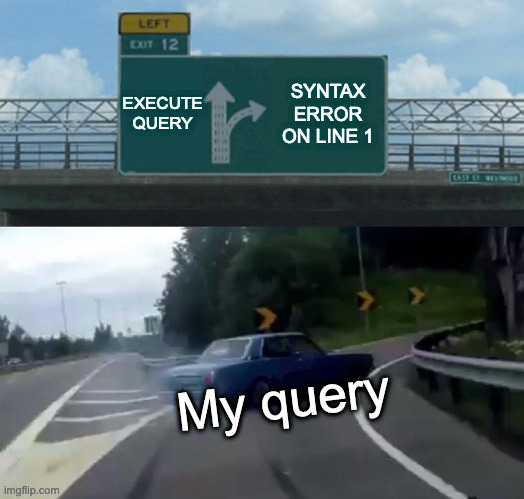
\includegraphics[width=0.4\textwidth]{images/syntaxerror.jpg}
\end{center}

\end{frame}

\begin{frame}
\frametitle{Steps Breakdown}
If so, then it will be validated to make sure that the attribute and relation names are valid inside the schema of the database being queried. 

Then this query is turned into a query tree or graph, which is used to devise the execution strategy. 

Then finally we can execute the query.

\end{frame}

\begin{frame}
\frametitle{Execution Steps Breakdown}
\begin{center}
	\includegraphics[width=0.9\textwidth]{images/query-processing-overview}
\end{center}

\end{frame}


\begin{frame}
\frametitle{Do Skip Steps!}

We will not spend time talking about the scanning, parsing, and verification steps of query processing.

A query with an error is rejected and  goes no further through the process. 

We therefore will give them no further consideration.

\end{frame}

\begin{frame}
\frametitle{Start with SQL}
Usually a query is expressed in SQL and that must then be translated into an equivalent relational algebra expression. 

Complex SQL queries are typically turned into \alert{query blocks}, which are translatable into relation algebra expressions. 

A query block has a single select-from-where expression, as well as related group-by and having clauses; nested queries are a separate query block.

\end{frame}

\begin{frame}
\frametitle{Select Your Choice}
A query like \texttt{SELECT salary FROM employee WHERE salary > 100000;} consists of one query block. 

The relational algebra for this expression is pretty easy to work out, and it gives us two possibilities. 

What are they?

\end{frame}

\begin{frame}
\frametitle{Select Your Choice}

We can select all tuples where salary is more than 100~000 and then perform a projection of the salary field of that result. 

The alternative is to do the projection of salary first and then perform the selection on the cut-down intermediate relation.

\end{frame}


\begin{frame}
\frametitle{Select with Subquery}

\texttt{SELECT name, street, city, province, postalCode FROM address WHERE id IN (SELECT addressID FROM employee WHERE department = 'Development');}. 

Then there are 2 query blocks, 1 for the subquery and 1 for the outer query. 

If there are multiple query blocks, then they do not have to follow the same strategy; they can be optimized separately if desired. 

\end{frame}


\begin{frame}
\frametitle{Make the Plan}


What we need instead is a \alert{query execution plan}.

\begin{center}
	
\includegraphics[width=0.5\textwidth]{images/blackadder.jpg}
\end{center}

\end{frame}


\begin{frame}
\frametitle{Make the Plan}


To build that up, each step of the plan needs annotations that specify how to evaluate the operation. 

This includes information such as what algorithm or what index to use. 

An algebraic operation with the associated annotations about how to get it done is called an \alert{evaluation primitive}. 

The sequence of these primitives forms the plan, that is, how exactly to execute the query.

\end{frame}

\begin{frame}
\frametitle{Time for Plan B}

If there are multiple possible way to carry out the plan, the system will need to make some assessment about which plan is the best. 

It is not expected that users will write optimal queries; instead the database server should choose the best approach via \alert{query optimization}. 

 The subject of query optimization is something we will also come back to.

\end{frame}

\begin{frame}
\frametitle{At What Cost?}

If you are asked to drive a car from point A to point B and there are multiple routes, you can evaluate your choices. 

To do so you need to break it down into different sections, such as drive along University Avenue, then get on Highway 85, then merge onto 401... 

By combining all of the segments, you get an estimate of how long that particular route will take. 

If you do this for all routes, you can see which route is the best. 

\end{frame}

\begin{frame}
\frametitle{Every Month is Bad Lane Change Month}

If there is a crash on the highway, traffic really sucks and your decision that taking this particular route would be fastest turns out to be wrong. 

\begin{center}
	
\includegraphics[width=0.4\textwidth]{images/traffic.jpg}
\end{center}

Short of being able to see into the future, this is more or less inevitable.

Estimates are just informed opinions and things may be worse (or better) than expected. 

\end{frame}

\begin{frame}
\frametitle{Execution Time}

Where does the time go in executing a query? 

The biggest component is most likely loading blocks from disk, considering how slow the disk operations are. 

In reality, CPU time is a nonzero part of query optimization, but we will ignore this for simplicity's sake and use only the disk accesses to assess cost.

\end{frame}

\begin{frame}
\frametitle{Think Disk}

The number of block transfers and the number of disk seeks are the important measures of interest here.
 
To compute the estimate of how long we think it will take to perform an operation, the formula is $b \times t_{T} + S \times t_{s}$. 

For a hard drive, transfer times are on the order of 0.1~ms and seek times are about 4~ms.

\end{frame}

\begin{frame}
\frametitle{Estimation Strategy Caveats}

Sometimes writes can be twice as expensive as reads. 

This is because the disk subsystem may read back the written data to check that the write succeeded, but we will assume that does not happen here. 

Similarly, at this first level we are not including the amount of time it takes to write a final result back. 

\end{frame}

\begin{frame}
\frametitle{Estimation Strategy Caveats}

We will imagine the worst case scenario, that is, only one block per relation can be in memory at a time. 

If we are ``wrong'' and the data we need is already in memory, the actual cost is less than the estimated cost (which is better than the reverse). 

\end{frame}



\begin{frame}
\frametitle{Estimates of Work}

The estimates calculate only the amount of work that we think it will take to complete the operation. 

Unfortunately, there are several factors that will potentially affect the actual wall-clock time it takes to carry out the plan:

\begin{itemize}
	\item How busy the system is
	\item What is in the buffer
	\item Data layout
\end{itemize}

You can probably think of various other factors.

\end{frame}

\begin{frame}
\frametitle{Estimates of Work}

Remember: the lowest cost approach is not necessarily the fastest!

\begin{center}
	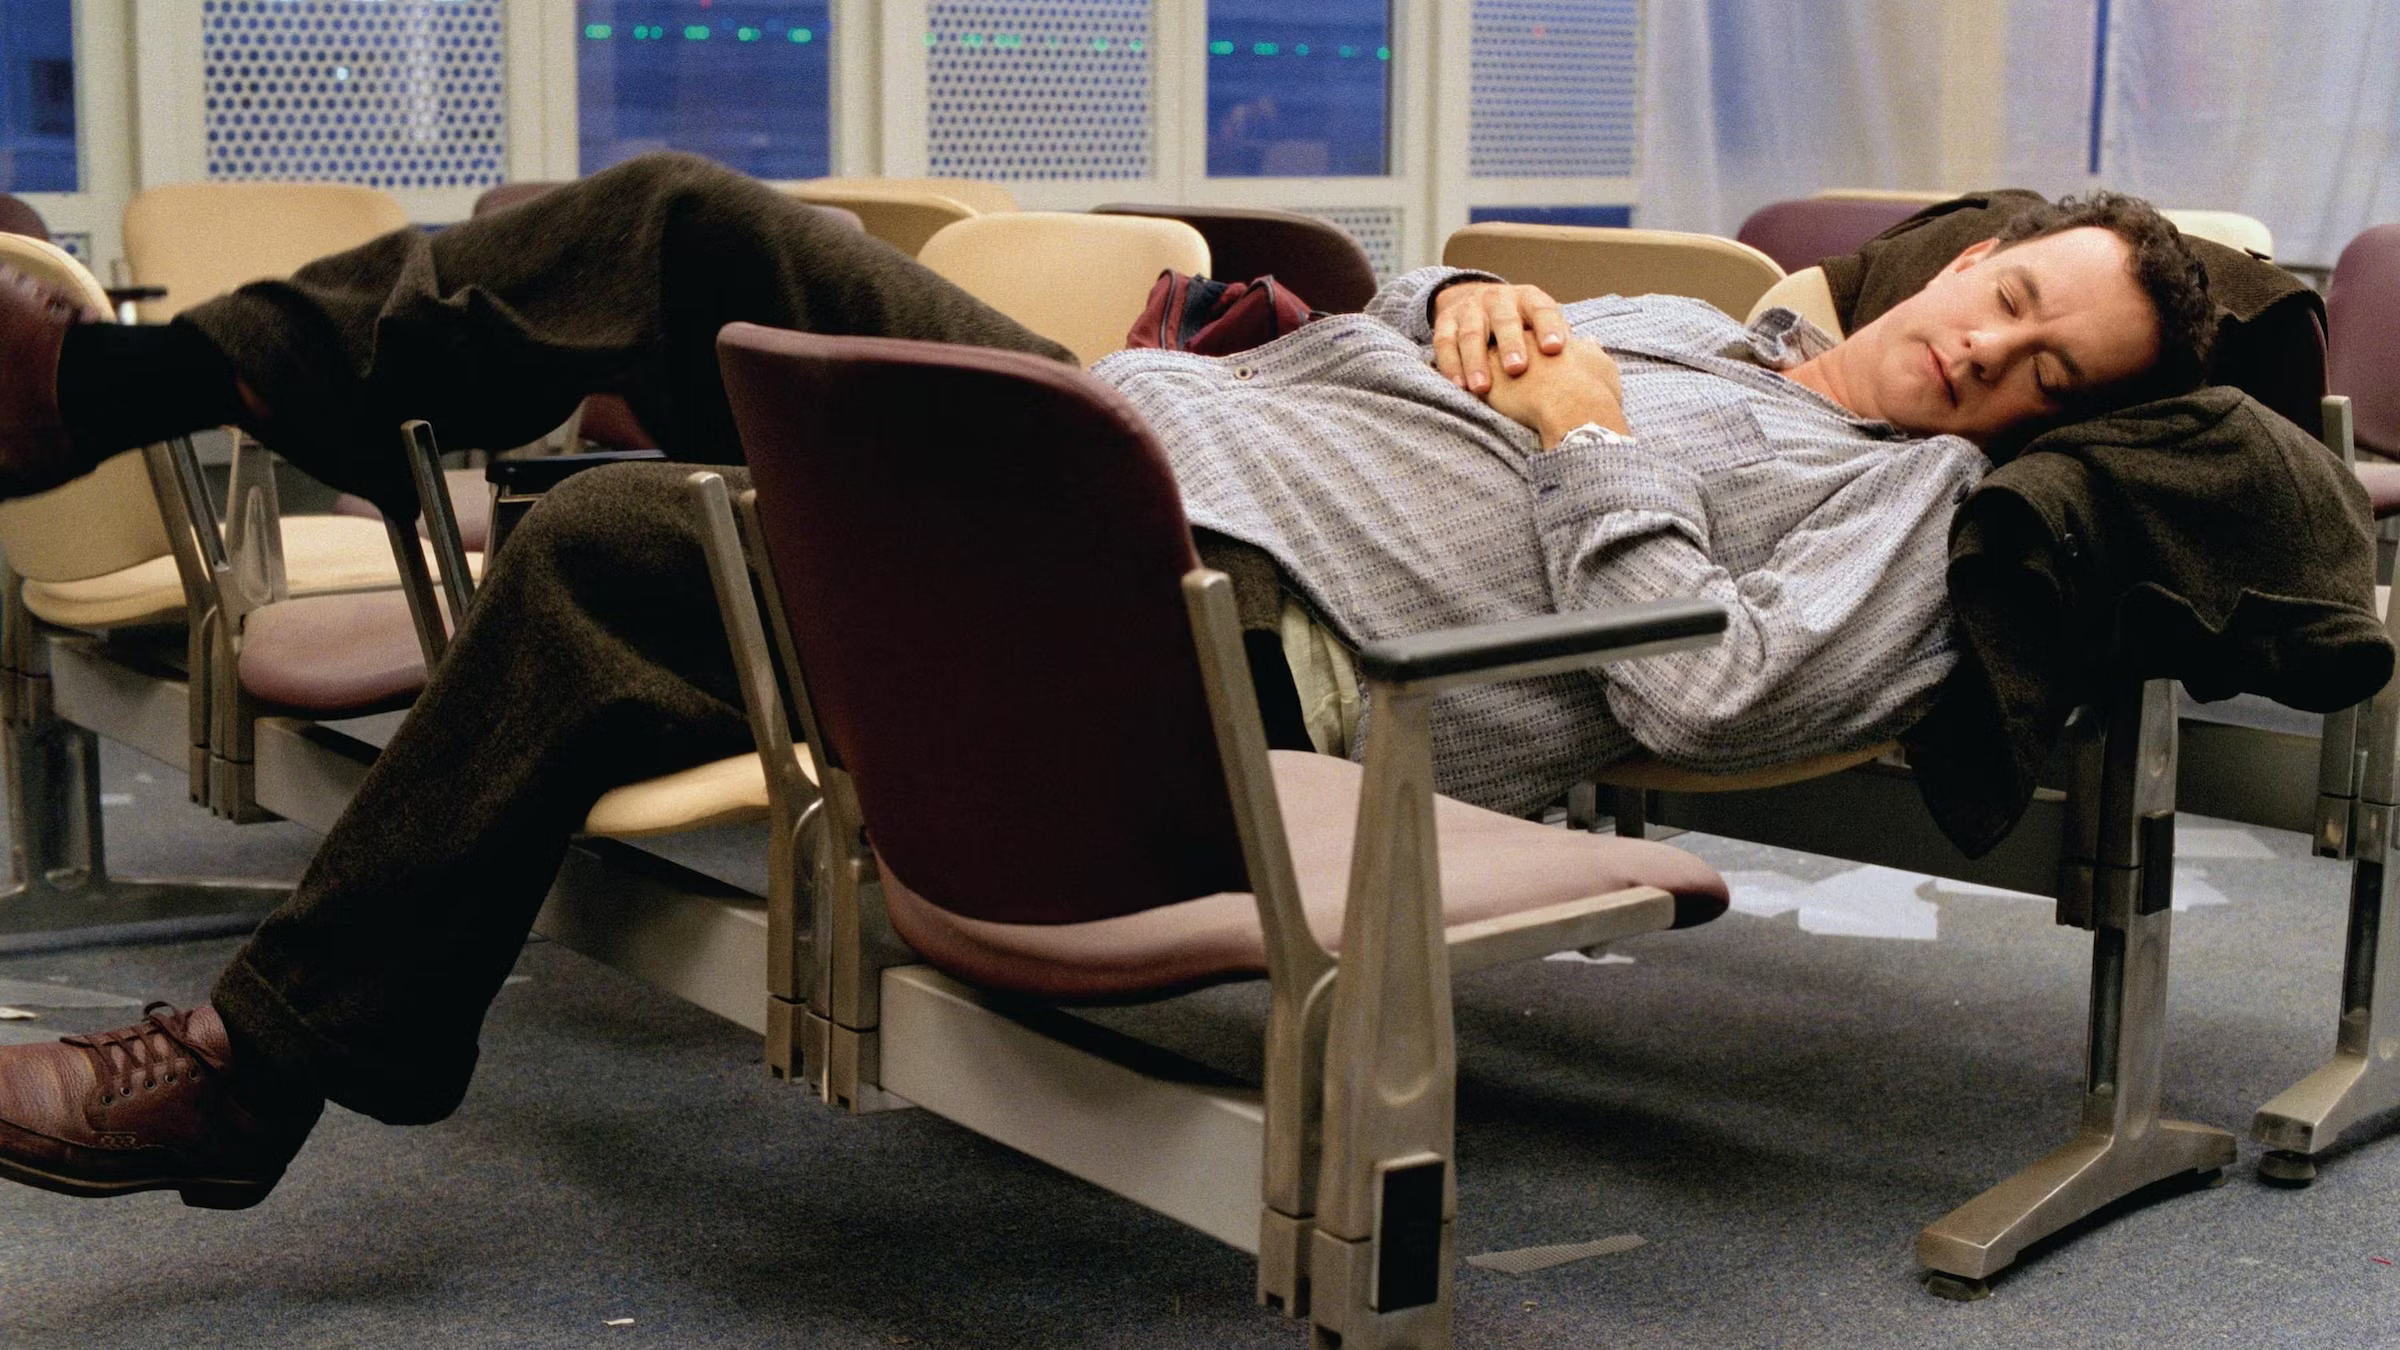
\includegraphics[width=0.75\textwidth]{images/terminal.jpg}
\end{center}

But the shorter connection time for the next flight cost \$50 more...

\end{frame}

\begin{frame}
\frametitle{Select Operation}

The first example for estimating cost: how to do a select operation. 

We will consider a lot of possibilities, some of which are obviously sub-optimal. 


Sometimes, a seemingly-terrible algorithm is our last resort, such as if we have to find something that has no index, we perform a linear search.


\end{frame}


\begin{frame}
\frametitle{Selection Scenario}

We have a select-from-where condition to be evaluated on a single relation.  

The relation is stored in 1 file and the file contains only records of that relation. 

The first approach is general and really needs no introduction.

\end{frame}



\begin{frame}
\frametitle{Select Strategy 1A: Linear Search}

The linear search is exactly what it sounds like.

We have only one seek to start reading the file, and then the transfer time for each block. 

Thus there is one seek plus one transfer for each block of the file and the cost estimate is $t_{s} + n \times t_{T}$ where $n$ is the number of blocks in the file.

This will work as a last resort if we have no other choice.

\end{frame}


\begin{frame}
\frametitle{Selection with Equality}

We would much prefer, if we can, to use an index of some sort.

If we have that, we can access fewer records than we would otherwise need to. 

The following group of strategies are applicable when the where condition contains an equality test, e.g., ``province equals Ontario''.

\end{frame}


\begin{frame}
\frametitle{Select Strategy 1B: Binary Search}

Binary search is also exactly what we are pretty well familiar with. 

If the file is ordered on something other than the primary key, and this is the where condition, we can search using a binary search algorithm. 

Binary search would then mean we can significantly reduce the number of blocks we need. 

But we will assume generally from here that we will look at B$^{+}$ trees.

\end{frame}

\begin{frame}
\frametitle{Select Strategy 2: Primary Index, Equality on Key}

If the select's where clause specifies equality on a primary index, i.e., the way the file is organized, it is very efficient. 

We traverse the tree to get to the leaf containing the pointer to the record. 

That means one seek and one transfer for each of the levels of the tree. 

Then we access the data directly, which is another seek and another transfer. 

The cost estimate is $(h_{i} + 1) \times (t_{s} + t_{T})$  ($h_{i}$ is the height of the index B$^{+}$ tree).

\end{frame}


\begin{frame}
\frametitle{Select Strategy 3: Primary Index, Equality on Non-Key}

If the primary index for the file is a non-key (non-unique) field then instead of getting one record we may get multiple records. 


The multiple records will be consecutive, because it is the primary index. 

Thus the cost will be $h_{i} \times (t_{s} + t_{T}) + b \times t_{T}$ where in this case $b$ is the number of block containing the target search key.

 Because the blocks with the actual data are stored sequentially we don't need to check the index again for the next ones, nor do we need to seek to them.
 
 Estimating $b$ can be somewhat difficult.

\end{frame}

\begin{frame}
\frametitle{Select Strategy 4: Secondary Index, Equality}
If the secondary index is on a unique field, then the cost estimate is the same as strategy 2:  $(h_{i} + 1) \times (t_{s} + t_{T})$.

If the key is not unique then the cost is higher. 

Unlike strategy 3, we cannot rely on the fact that the records are consecutive.

We make the opposite assumption, that each record requires a seek and a transfer of a new block. 

This the estimate is $(h_{i} + k) \times (t_{s} + t_{T})$ where $k$ is the number of records matching the condition.

As with $b$ in strategy 3, estimating the value of $k$ is probably difficult.


\end{frame}



\begin{frame}
\frametitle{Selection with Comparison}

Until this point we just handled an equality condition, where we looked for an exact match. 

A comparison is more complex. 

We can still use the linear search approach, if we must, but if we have an index we may still prefer to use that. 

We will continue to assume that the file index is organized in a B$^{+}$ tree.

\end{frame}

\begin{frame}
\frametitle{Select Strategy 5: Primary Index, Comparison}

Suppose our desired search value is $x$. 

If the attribute being compared is $A$, then our possibilities are\\
\quad (1) $A > x$ or $A \geq x$,\\
\quad (2) $A < x$ or $A \leq x$.

For the first case, we use the tree to go to the first tuple where $A = x$ or $A > v$ respectively. 

Then we do a file scan from start to the end of the file. In that case, our cost estimates are like those of strategy 3.
\end{frame}

\begin{frame}
\frametitle{Select Strategy 5: Primary Index, Comparison}

For the second case, we start at the beginning of the file and go until the first tuple with $A = x$ or $A > x$ respectively. 

This is more or less a linear scan that may end early.

When doing this comparison, the index contributed absolutely nothing.


\end{frame}


\begin{frame}
\frametitle{Select Strategy 6: Secondary Index, Comparison}

This case resembles the case of strategy 4, equality on a non-key field. 

Fetching the actual data is a pain, of course. 

If the number of records to be fetched is large, because of all the jumping back and forth, it might actually be worse than simply performing a linear search.  

It depends on the value of $k$, how many records will match. 

\end{frame}


\begin{frame}
\frametitle{Complex Selection}

Previous strategies, except linear search, assumed the predicate had 1 clause. 

Before we start, a review of the ideas of conjunction, disjunction, and negation.

A conjunctive selection involves the logical AND operation.

A disjunctive selection involves the logical OR operation. 

A negation selection $\sigma_{\neg \theta}(r)$ is the set of all tuples of $r$ for which the condition $\theta$ evaluates to false. 

\end{frame}

\begin{frame}
\frametitle{Select Strategy 7: Conjunction, One Index}
We will first find all records that satisfy one of the simple conditions, and then throw away any of the retrieved that do not match the remaining conditions. 

One of the previous strategies (2 through 6) will suffice, and the cost is pretty much determined by which of those strategies is used. 

We would take estimates for each strategy and choose the one with the lowest expected cost.

\end{frame}



\begin{frame}
\frametitle{Select Strategy 7: Conjunction, One Index}
Ah, but which simple condition do we choose? 

If only one has an index, then we use the one index. That was easy. 

If there are multiple choices, ideally we choose the most restrictive -- the one that will match the fewest tuples. 

\end{frame}



\begin{frame}
\frametitle{Select Strategy 8: Conjunction, Composite Index}
Recall from the discussion of indexing that a composite index is one that is on multiple attributes. 

If the selection has multiple simple conditions, a subset of which exist in a composite index on the relation, that is very helpful. 

Then we can use the index directly. 

If the complex where predicate is exactly equal to the composite index, we will be using one of strategies 2, 3, or 4. 

If there are some conditions that form the composite index and others that do not, our strategy looks more like strategy 7.

\end{frame}

\begin{frame}
\frametitle{Select Strategy 9: Conjunction, Intersection}
Another way we could do the conjunction: look at the record pointers. 

We get a list of record pointers for each simple condition that has an index and compute the intersection of these. 

If there are any conditions on attributes without an index, then we must look through the results to throw away those records that don't meet all conditions.

The cost here is the sum of the cost of looking through each index, plus the cost of loading the records after the intersection is computed. 

\end{frame}

\begin{frame}
\frametitle{Select Strategy 10: Disjunction, Union}
Much like the conjunction strategy, we get a list of record pointers for each of the conditions where there is an index. 

Instead of computing the intersection, we find the union (no duplicates) of these pointers. 

Sorting may make the disk reads closer and speed things along.

If there is at least one condition that does not have an index, then it is makes sense to just linear scan since we are going to have to do that anyway.

\end{frame}

\begin{frame}
\frametitle{Select Strategy 11: Negation}

Although one can, of course, do a linear scan to find those that, unlike usual, do NOT meet the given conditions, what can one do? 

If we have an index on the field that might help: we can evaluate the index and decide which records match the not condition, and only load those. 

As the last resort, the linear search approach will be necessary.

\end{frame}

\end{document}

